\FloatBarrier
\section{SIMD Experiments}
\label{sec:SIMDExperiments}
Section~\ref{sec:SIMDImpl} describes how to use the new SSE4.1 instruction set to speed up the operation of data-oblivious sorting algorithms.
In this section, we show how performance is affected in real-life implementations of the algorithms, and show how different usages of the SIMD architecture can make or break the performance gain.
These experiments we focus on the instruction count and running time, as these are the only metrics that change noticeably when using SSE.

Note that performing two recursive calls in a single scan is not beneficial when using SIMD, so Odd-Even Mergesort will only use the simple buffering strategy.

\subsection{Instructions}

The immediate effect of using SSE instructions is a significant reduction in the amount of operations required per comparison, due to having 4-way comparisons and intrinsic \texttt{min}/\texttt{max} operations. Figure~\ref{fig:SIMD:instructions} and~\ref{fig:SIMD:instructions:comparisons} show the total amount of instructions, and the number of instructions per comparison.

Both Randomized Shellsort and Odd-Even Mergesort show a reasonable reduction in instruction count, but overhead from the general operations of the algorithms overshadow the amount of operations tied up comparisons.

Bitonic Sort shows a massive reduction in instruction count from the application of SIMD instructions. The massive gain for Bitonic Sort stems from the low instruction overhead of the algorithm, since the benefit of using SIMD is heavily dependent on the amount of operations dedicated to comparisons.

Pratt's Shellsort and Shaker Sort also both show a big impact from SIMD in the number of instructions performed. This big reduction in the amount of instructions is most likely caused by the structure of the algorithms being based entirely on nested for-loops. No extra instructions are spent setting up recursive calls. Especially noteworthy is the low instruction count of Shaker Sort, combined with an $O(n \log n)$ running time.

\begin{figure}
\center
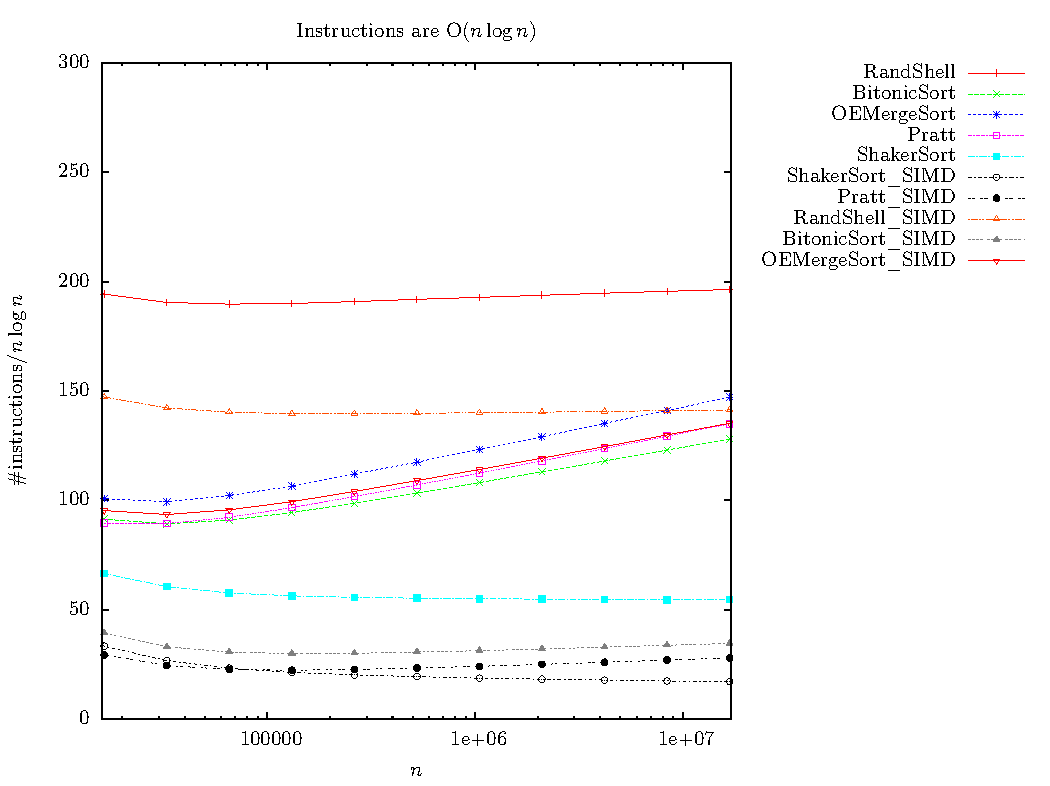
\includegraphics[width=\textwidth]{graphs/SIMD/nlogninstructions.pdf}
\caption{Instruction count with and without SIMD}
\label{fig:SIMD:instructions}
\end{figure}


\begin{figure}
\center
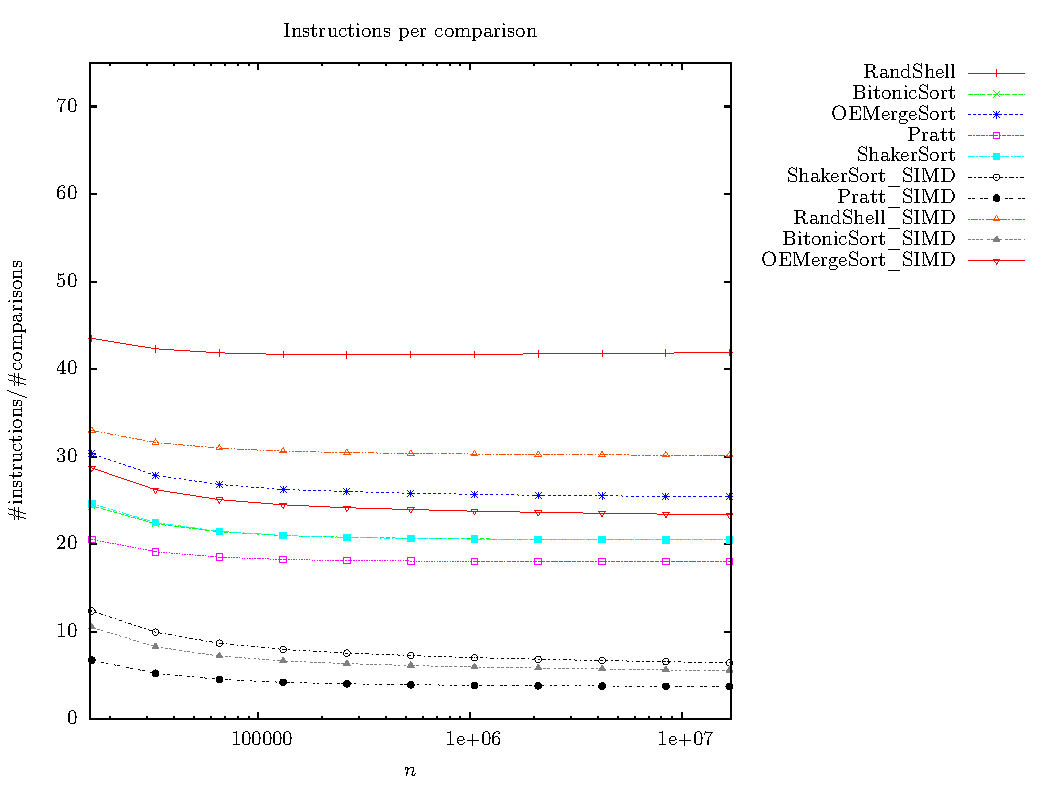
\includegraphics[width=\textwidth]{graphs/SIMD/instructionscomparison.pdf}
\caption{Instructions per comparison count with and without SIMD}
\label{fig:SIMD:instructions:comparisons}
\end{figure}

\subsection{Time}

Having shown the impact on the instruction count when using SSE operations, let us consider the actual performance gain.

In Figure~\ref{fig:SIMD:time} we can see the actual running times, while Figure~\ref{fig:SIMD:timediff} shows the performance gain. Table~\ref{tab:SIMD:timediffavg} shows the mean performance gain, as obtained from the data shown in Figure~\ref{fig:SIMD:timediff}.

Randomized Shellsort shows a small but noticeable gain from SSE instructions. The problem of using SIMD with Randomized Shellsort comes from the need to fetch data into the SSE registers from separate locations in the memory due to the random nature of the region comparison procedure.

Odd-Even Mergesort shows a small but noticeable improvement from SSE instructions. Odd-Even Mergesort has much more linear memory access patterns than Randomized Shellsort, but they are unfortunately often shifted away from 16-byte boundaries of memory, which prevents optimal SSE load behaviour. 

Bitonic Sort shows a massive improvement in running time when using SSE instructions. This stems from the low overhead of the algorithm, coupled with fully linear 16-byte aligned memory access patterns. 

Shaker Sort shows a low running time, and a good improvement in running time from utilizing SSE instructions. Pratt's Shellsort also shows a good utilization of SIMD, but degrades rapidly at the cache limit on large inputs. Figure~\ref{fig:SIMD:timediff} also shows an unstable impact of SIMD to Pratt's Shellsort. We have no evidence pointing to a single source causing the degradation in Pratt's Shellsort at larger input sizes, but the fact that Shaker Sort shows a similar but smaller impact at a similar size, which lies close to the cache limit, suggests un-aligned SIMD accesses outside of the cache as a possible cause. The sizes of the subsequences processed by Pratt's Shellsort are not monotonically ascending, as they are for Shaker Sort, and this causes the algorithm to continously switch between SIMD and sequential execution, which is another possible cause for the degradation in performance.

\begin{table}[!h]
\begin{adjustwidth}{-.5in}{-.5in}
\centering
\begin{tabular}{|l|c|c|c|c|c|}
\hline
Algorithm & Randomized Shellsort & Bitonic Sort & Odd-Even Mergesort & Pratt & Shaker Sort \\ \hline
Factor    & 1.08                 & 2.81         & 1.12 & \textcolor{red}{2.87} & \textcolor{red}{2.16}              \\ \hline
\end{tabular}
\caption{Mean gain from SSE}
\label{tab:SIMD:timediffavg}
    \end{adjustwidth}
\end{table}

\begin{figure}
\center
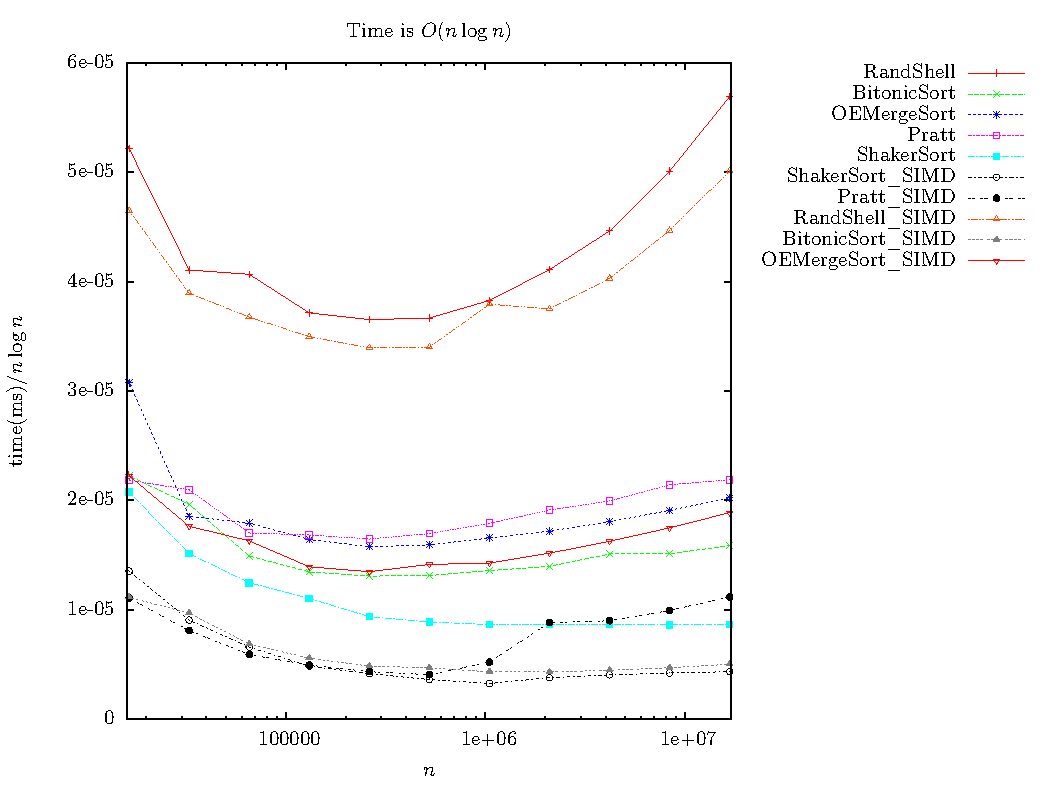
\includegraphics[width=\textwidth]{graphs/SIMD/nlogntime.pdf}
\caption{Time with and without SIMD}
\label{fig:SIMD:time}
\end{figure}


\begin{figure}
\center
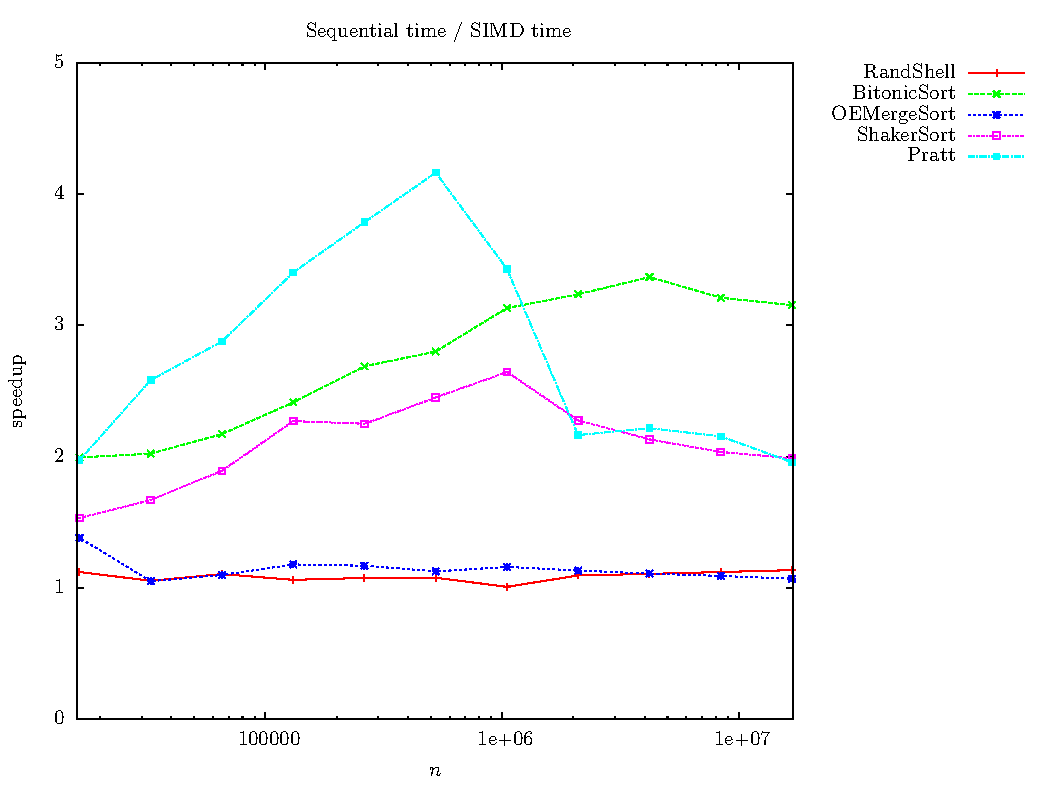
\includegraphics[width=\textwidth]{graphs/SIMD/timediff.pdf}
\caption{Time factor with and without SIMD}
\label{fig:SIMD:timediff}
\end{figure}

